\documentclass[conference]{IEEEtran}
\IEEEoverridecommandlockouts

\usepackage{cite}
\usepackage{amsmath,amssymb,amsfonts}
\usepackage{algorithmic}
\usepackage{graphicx}
\usepackage{textcomp}
\usepackage{xcolor}
\usepackage{booktabs}
\usepackage{array}
\usepackage{url}

\def\BibTeX{{\rm B\kern-.05em{\sc i\kern-.025em b}\kern-.08em
    T\kern-.1667em\lower.7ex\hbox{E}\kern-.125emX}}

\begin{document}

\title{Making SQL Query Optimization Explainable}

\author{
\IEEEauthorblockN{\begin{tabular}{@{}>{\centering\arraybackslash}p{0.24\textwidth}>{\centering\arraybackslash}p{0.24\textwidth}>{\centering\arraybackslash}p{0.24\textwidth}>{\centering\arraybackslash}p{0.24\textwidth}@{}}
Manuela Gu\'edez & Guillermo Tula & Bernardo Rychtenberg & Fiorella Cravero
\end{tabular}}
\IEEEauthorblockA{\begin{tabular}{@{}>{\centering\arraybackslash}p{0.24\textwidth}>{\centering\arraybackslash}p{0.24\textwidth}>{\centering\arraybackslash}p{0.24\textwidth}>{\centering\arraybackslash}p{0.24\textwidth}@{}}
\textit{Dept. de Informática e IA} & \textit{Dept. de Informática e IA} & \textit{Dept. de Informática e IA} & \textit{Dept. de Informática e IA} \\
\textit{Universidad Católica de Uruguay} & \textit{Universidad Católica de Uruguay} & \textit{Universidad Católica de Uruguay} & \textit{Universidad Católica de Uruguay} \\
Montevideo, Uruguay & Montevideo, Uruguay & Montevideo, Uruguay & Montevideo, Uruguay \\
\url{manuela.guedez@ucu.edu.uy} & \url{guillermo.tula@correo.ucu.edu.uy} & \url{brychtenberg@ucu.edu.uy} & \url{fiorella.cravero@ucu.edu.uy}
\end{tabular}}
}



\maketitle

\begin{abstract}
Cost-based SQL query optimizers select execution plans from a large combinatorial search space, yet the factors driving these decisions remain largely opaque. This paper presents an Explainable Artificial Intelligence (XAI) framework that vectorizes candidate plans and uses a local Ridge proxy with SHAP to explain optimizer-estimated cost. It produces global importance rankings, local waterfall explanations, and natural-language summaries. The extended evaluation covers 112 templates with one to six tables over five seeds, three dataset sizes, and three distributions. Out-of-query fidelity reached mean $R^2$ values of 0.993 for Selinger and 0.996--1.000 for BayesCard; SHAP stability is reported with bootstrap 95\% confidence intervals. The study remains a proof of concept on a controlled synthetic workload; production-scale evaluation and DBA validation remain future work.
\end{abstract}

\begin{IEEEkeywords}
SQL, XAI, Query Optimization, SHAP, Explainability.
\end{IEEEkeywords}

\section{Introduction}

The continuous growth in data volume and query complexity has made efficient query processing a central requirement of modern database systems, with query optimizers responsible for selecting, among a combinatorial space of semantically equivalent execution plans, the one expected to minimize resource consumption and/or response time. This problem has been central to relational database engineering since the seminal work of System R \cite{b1}, which established the paradigm of searching over alternative join orders and access paths guided by cost estimation. Even for relatively simple queries, the number of alternative plans arising from different join orders, access methods, and operator implementations grows in a combinatorial way, so modern optimizers cannot exhaustively evaluate every alternative. Instead, they rely on heuristics, pruning strategies, and cost estimation models \cite{b2,b3}. However, cardinality estimation errors remain a primary cause of suboptimal query plans \cite{b4}, leading to unpredictable performance degradation \cite{b5}.

To improve accuracy, modern database research has explored probabilistic approaches \cite{b6} and machine learning models for cardinality estimation \cite{b7} and query optimization \cite{b8}. Despite promising results, evaluating the real-world readiness of these learned models is challenging \cite{b9}. Recent frameworks such as BayesCard \cite{b10} revitalize cardinality estimation through probabilistic graphical models trained on the underlying data, offering a balance between accuracy and structural transparency.

While these approaches enable practical optimization times, they also make optimizer decisions difficult to understand and interpret. Database administrators (DBAs) and researchers often have limited visibility into why a particular plan was selected over competing alternatives, or which query and data characteristics had the greatest influence on that decision. This opacity persists even for expert developers, a problem exacerbated by the increasing use of complex machine learning components in databases.

Recent advances in Explainable Artificial Intelligence (XAI) provide promising tools for addressing this limitation \cite{b11}. While methods such as LIME \cite{b12} provide local approximations, feature attribution methods based on game theory offer consistent insights into the underlying decision-making process.

This work investigates the application of SHapley Additive exPlanations (SHAP) \cite{b13} to SQL query optimization. The central hypothesis is that understanding which query and data characteristics most strongly influence an optimizer's cost-based decisions can improve transparency, facilitate debugging and analysis of optimizer behavior, and ultimately inform the design of more interpretable query optimization strategies. The study does not evaluate whether the framework improves DBA productivity or decision quality; such claims require a controlled study with database professionals.

\begin{figure*}[!t]
    \centering
    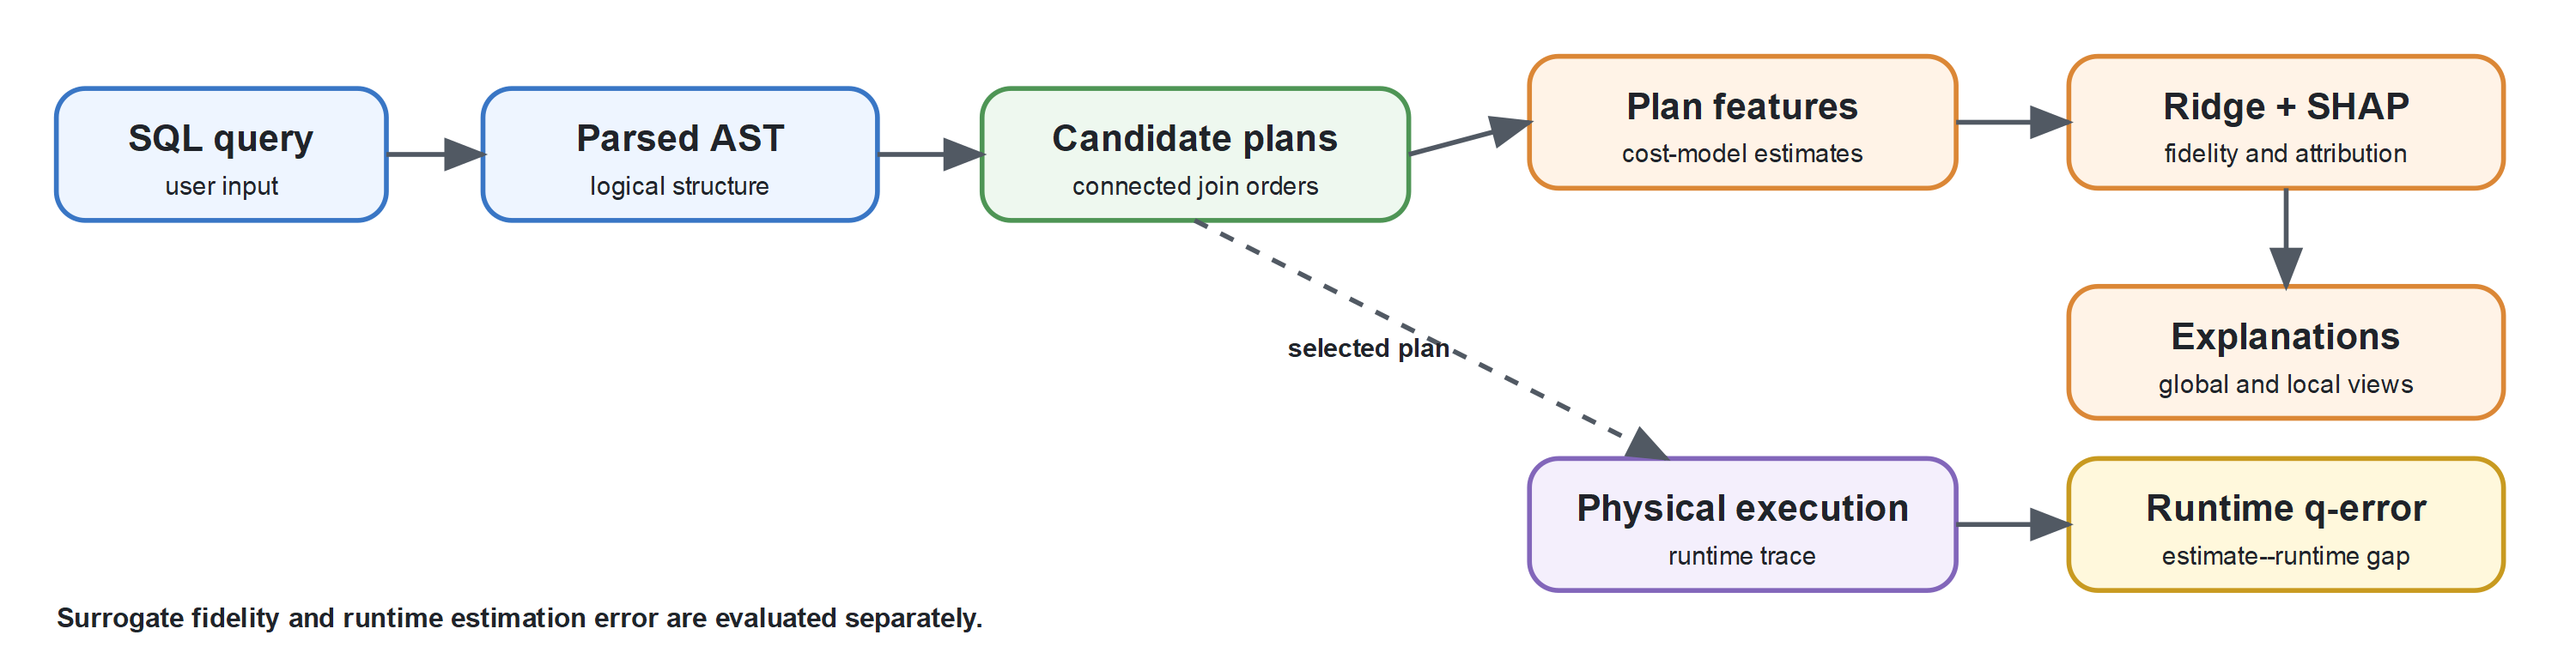
\includegraphics[width=0.96\textwidth]{fig1_framework.png}
    \caption{Architecture of the explainability framework. The query-processing pipeline generates candidate plans and estimated plan features. The explainability pipeline trains and evaluates a Ridge surrogate and computes SHAP attributions. Runtime traces are analyzed separately through q-error to assess cardinality-estimation discrepancies; they are not used as a measure of surrogate fidelity.}
    \label{fig:framework}
\end{figure*}

\section{Materials and Methods}

Fig.~\ref{fig:framework} presents the overall architecture of the explainability framework, illustrating the relationship between query processing, feature attribution, and runtime analysis.

\subsection{Query Processing and Optimizers}

Query processing in this work refers to the complete workflow that transforms an input SQL query into a set of candidate execution plans. Each query is first parsed and represented as an Abstract Syntax Tree (AST), preserving its logical semantics while enabling the system to explore alternative physical strategies. The optimizer explores connected left-deep join orders, estimates the cost of each candidate using available statistics, and selects the plan expected to minimize execution work.

Two cost-based optimization paradigms are considered. The classical Selinger-style baseline uses catalog row counts and distinct values with dynamic programming and may choose any base relation, exploring up to $2(N-1)!$ connected orders in the star schema. BayesCard \cite{b10} uses Bayesian selectivity profiles with catalog fallback, fixes the original \texttt{FROM} table, and explores up to $(N-1)!$ orders. Both exclude Cartesian intermediates and cap six-table enumeration at 50 candidate plans. Learned, adaptive, production, and reinforcement-learning optimizers such as \cite{b14} remain outside the present scope and are left for future work.


\subsection{Plan Vectorization}

The optimizer operates over an AST representation of each candidate plan. Although the AST fully describes the optimizer's decision process, it cannot be directly used by numerical feature-attribution methods such as SHAP. Plan vectorization bridges this gap by mapping each optimized AST to a structured numerical feature vector.

For each candidate plan, the extracted vector includes structural characteristics, initial table cardinalities, predicate and join selectivities, intermediate result sizes after each join, and accumulated estimated work. These variables, summarized in Table~\ref{tab:features}, constitute the vocabulary through which optimizer decisions are explained.

\begin{table}[htbp]
\caption{Main plan-level features used for explanation}
\label{tab:features}
\centering
\footnotesize
\begin{tabular}{p{0.36\columnwidth} p{0.53\columnwidth}}
\toprule
\textbf{Feature} & \textbf{Description} \\
\midrule
\texttt{table\_count} & Number of tables in the query plan \\
\texttt{predicate\_count} & Number of predicates in the query \\
\texttt{base\_filtered\_rows} & Estimated rows after base-table filtering \\
\texttt{join\_N\_table\_rows} & Estimated rows of the table added at join step $N$ \\
\texttt{join\_N\_selectivity} & Estimated selectivity of join step $N$ \\
\texttt{join\_N\_output\_rows} & Estimated intermediate rows after join step $N$ \\
\texttt{sum\_intermediate\_rows} & Accumulated estimated intermediate rows \\
\texttt{estimated\_cost} & Surrogate target; excluded from predictors \\
\bottomrule
\end{tabular}
\end{table}

\subsection{Explainability Pipeline}

The XAI module generates alternative join orders and records the selected plan and runner-up alternatives. A lightweight Ridge proxy is trained on the candidates of the query under analysis, preserving the local nature of the original explanation. Numeric features and costs are transformed using $\log(1+x)$.

SHAP assigns each feature a contribution to estimated cost. Local explanations describe the selected plan and closest alternative, while global importance aggregates mean absolute contributions. An additional Ridge evaluation measures out-of-query fidelity with GroupKFold grouped by query; it does not replace the local proxy used for explanations.

Beyond raw SHAP values, an LLM receives the already computed plan identifiers, costs, feature values, and SHAP contributions and generates an executive summary, the main positive and negative drivers, and a runner-up comparison. It is only a communication layer: it does not select plans, estimate costs, fit Ridge, or compute SHAP. Its output is not experimental evidence and was not evaluated with DBAs.

SHAP was selected because its additive contributions support both plan-level explanations and aggregation across repeated experiments. LIME is primarily local and depends on its perturbations, kernel, and neighborhood \cite{b12}. Since this study also requires global importance and stability analysis, SHAP is the principal method; systematic comparison with LIME remains future work.

\section{Experimental Setup}

\subsection{Synthetic Database and Workload}

A controlled synthetic database uses a six-table star schema with one fact table and five dimensions. The generator produces 277 unique templates; the reference experiment uses a deterministic stratified subset of 112: 12 single-table queries and 20 for each table count from two to six. Queries contain zero to five joins and zero to two predicates, including conjunction and disjunction variants.

Five seeds are evaluated for fact-table sizes of 300, 1,000, and 3,000 rows and for uniform, Zipf-like skewed, and correlated distributions, yielding 45 configurations per optimizer. Each run uses an isolated catalog. Table~\ref{tab:workload} summarizes workload structure, cardinalities, and candidate counts.

\begin{table}[!t]
\caption{Workload composition, plans, and cardinalities}
\label{tab:workload}
\centering
\scriptsize
\begin{tabular}{rrrrrr}
\toprule
\multicolumn{6}{c}{\textit{(a) Query templates and candidate plans per query}}\\
\textbf{Tables} & \textbf{Joins} & \textbf{Templates} & \textbf{Pred.} & \textbf{Sel.} & \textbf{Bayes} \\
\midrule
1 & 0 & 12 & 0--2 & 1 & 1 \\
2 & 1 & 20 & 0--2 & 2 & 1 \\
3 & 2 & 20 & 0--2 & 4 & 2 \\
4 & 3 & 20 & 0--2 & 12 & 6 \\
5 & 4 & 20 & 0--2 & 48 & 24 \\
6 & 5 & 20 & 0--2 & 50 & 50 \\
\midrule
\multicolumn{6}{c}{\textit{(b) Relation cardinalities by dataset size}}\\
\textbf{Relation} & \multicolumn{2}{c}{\textbf{Small}} & \textbf{Medium} & \multicolumn{2}{c}{\textbf{Large}}\\
\midrule
Fact & \multicolumn{2}{c}{300} & 1,000 & \multicolumn{2}{c}{3,000}\\
Departments & \multicolumn{2}{c}{4} & 13 & \multicolumn{2}{c}{20}\\
Locations & \multicolumn{2}{c}{15} & 50 & \multicolumn{2}{c}{100}\\
Employees & \multicolumn{2}{c}{30} & 100 & \multicolumn{2}{c}{200}\\
Projects & \multicolumn{2}{c}{10} & 33 & \multicolumn{2}{c}{80}\\
Categories & \multicolumn{2}{c}{3} & 10 & \multicolumn{2}{c}{20}\\
\bottomrule
\end{tabular}
\end{table}

\subsection{Evaluation Metrics}

\subsubsection{Surrogate Fidelity}
Ridge fidelity is reported with $R^2$, MAE in log and original cost space, normalized original-cost MAE, Spearman correlation, Kendall's $\tau$, and top-1 agreement between the optimizer's and surrogate's minimum-cost plans.

Queries whose candidate plans have identical target costs are excluded from rank-based metrics because no target ordering exists. They remain included in $R^2$ and MAE. Per-run confidence intervals are calculated by bootstrap resampling complete queries rather than individual plans.

\subsubsection{SHAP Stability}
Statistical stability is evaluated over five independently generated dataset seeds and the three sizes and distributions. For every query and feature, the analysis reports normalized mean absolute SHAP importance, standard deviation, bootstrap 95\% confidence interval, mean rank, and top-5 frequency. Paper-level summaries aggregate seed-level means only after preserving the per-query measurements.

\subsubsection{Runtime Q-error}
Runtime traces are analyzed separately from surrogate fidelity. For an optimizer-estimated quantity $\hat{x}$ and the corresponding observed runtime quantity $x$, q-error is defined as
\begin{equation}
q\text{-error}=\max\left(\frac{\hat{x}}{x},\frac{x}{\hat{x}}\right).
\end{equation}
A q-error of 1 indicates exact agreement. Larger values indicate a greater discrepancy between the optimizer's estimate and observed execution. This metric assesses whether influential estimated features, such as intermediate result sizes, correspond to the quantities observed during execution. It is distinct from Ridge surrogate fidelity.

\section{Results and Discussion}

\begin{figure*}[!t]
  \centering
  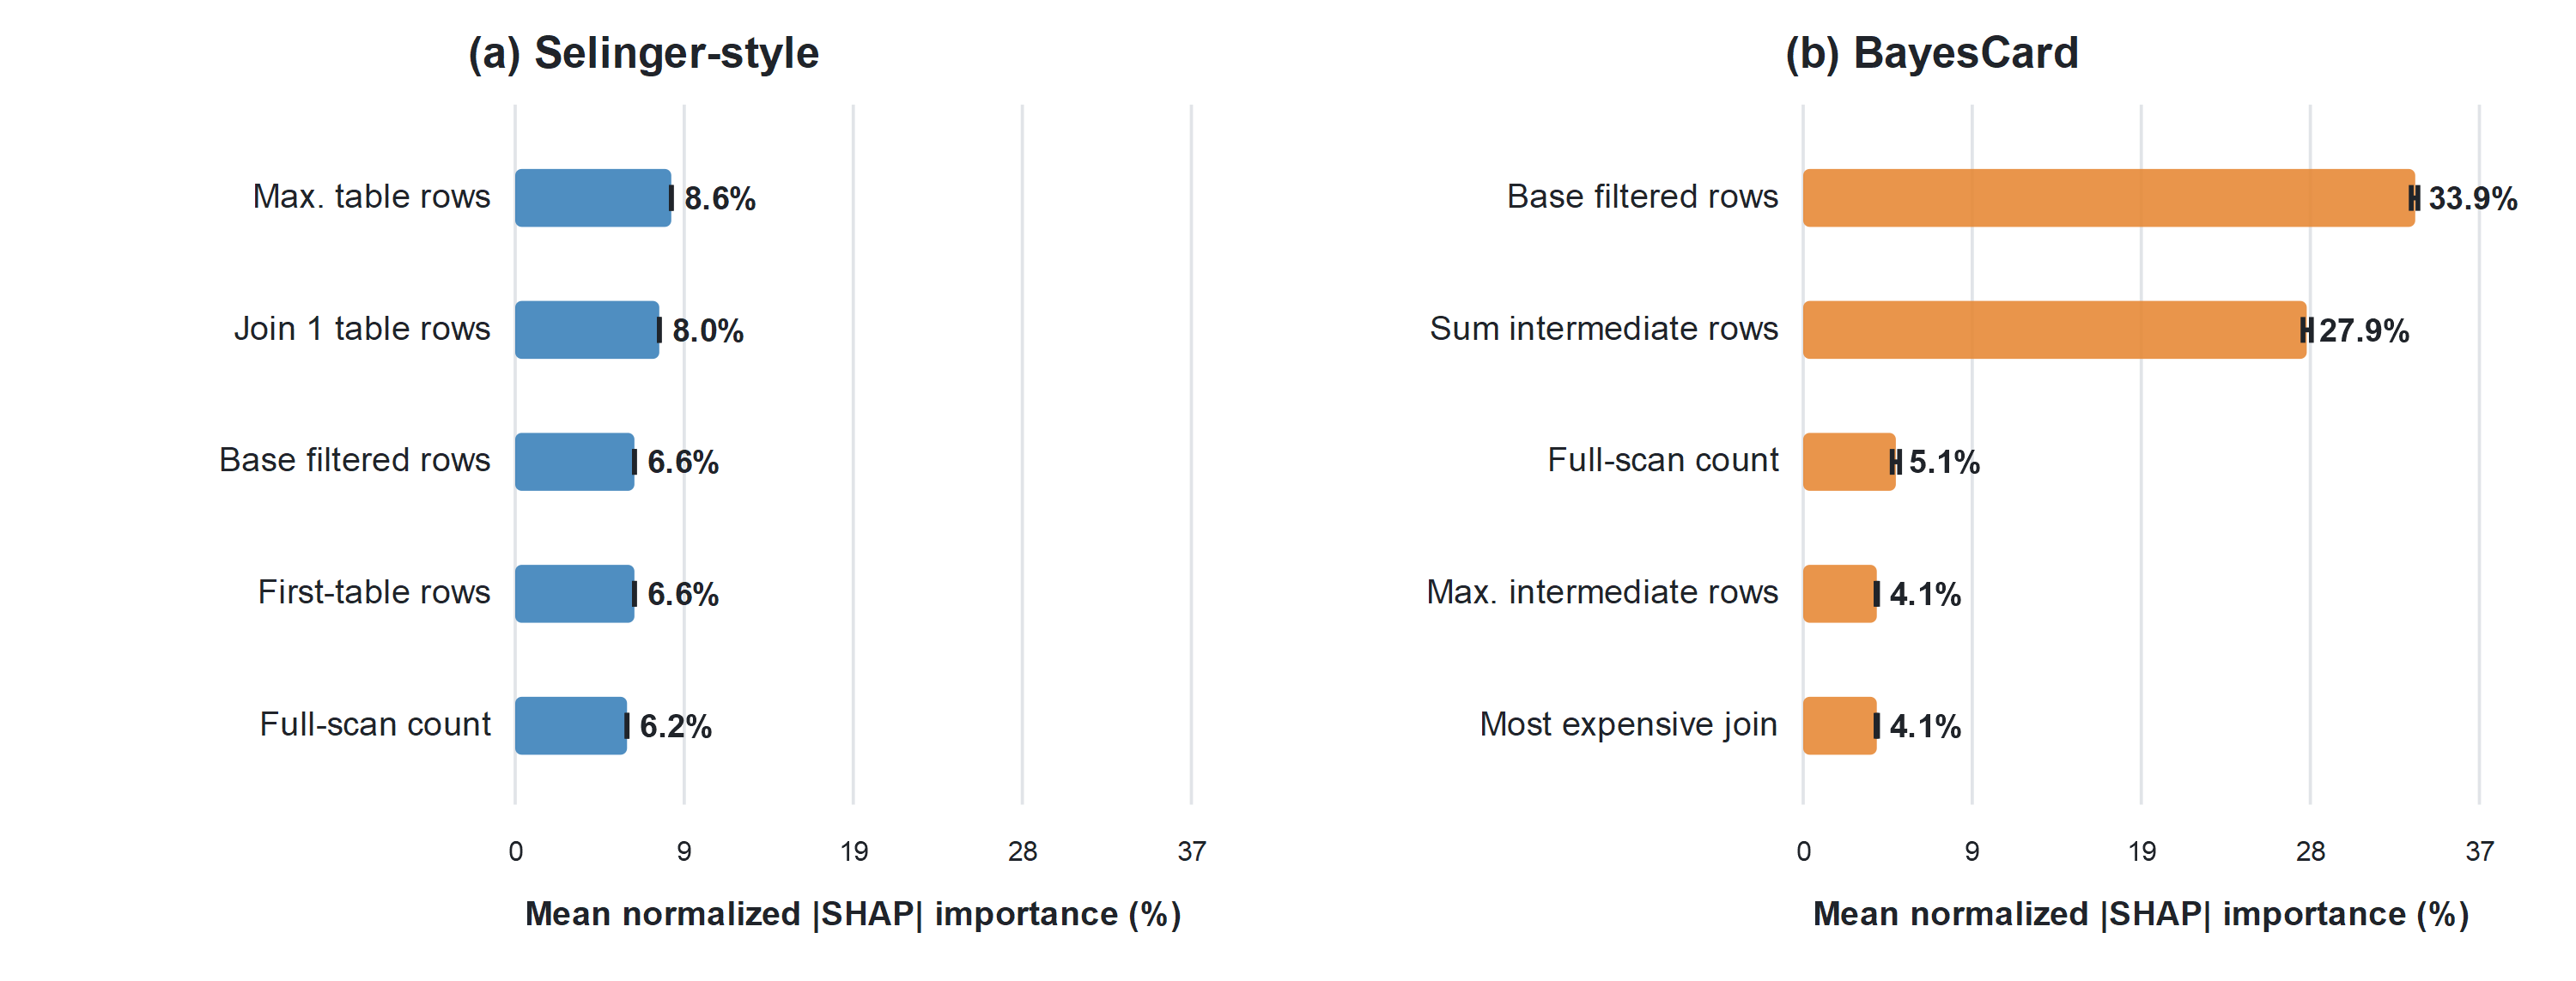
\includegraphics[width=0.90\textwidth]{fig2_global_shap.png}
  \caption{Global SHAP importance under the final protocol. Bars show mean normalized absolute importance; error bars show bootstrap 95\% confidence intervals over five seed-level means after averaging queries, sizes, and distributions within each seed.}
  \label{fig:shap_stability}
\end{figure*}

\begin{figure*}[!t]
  \centering
  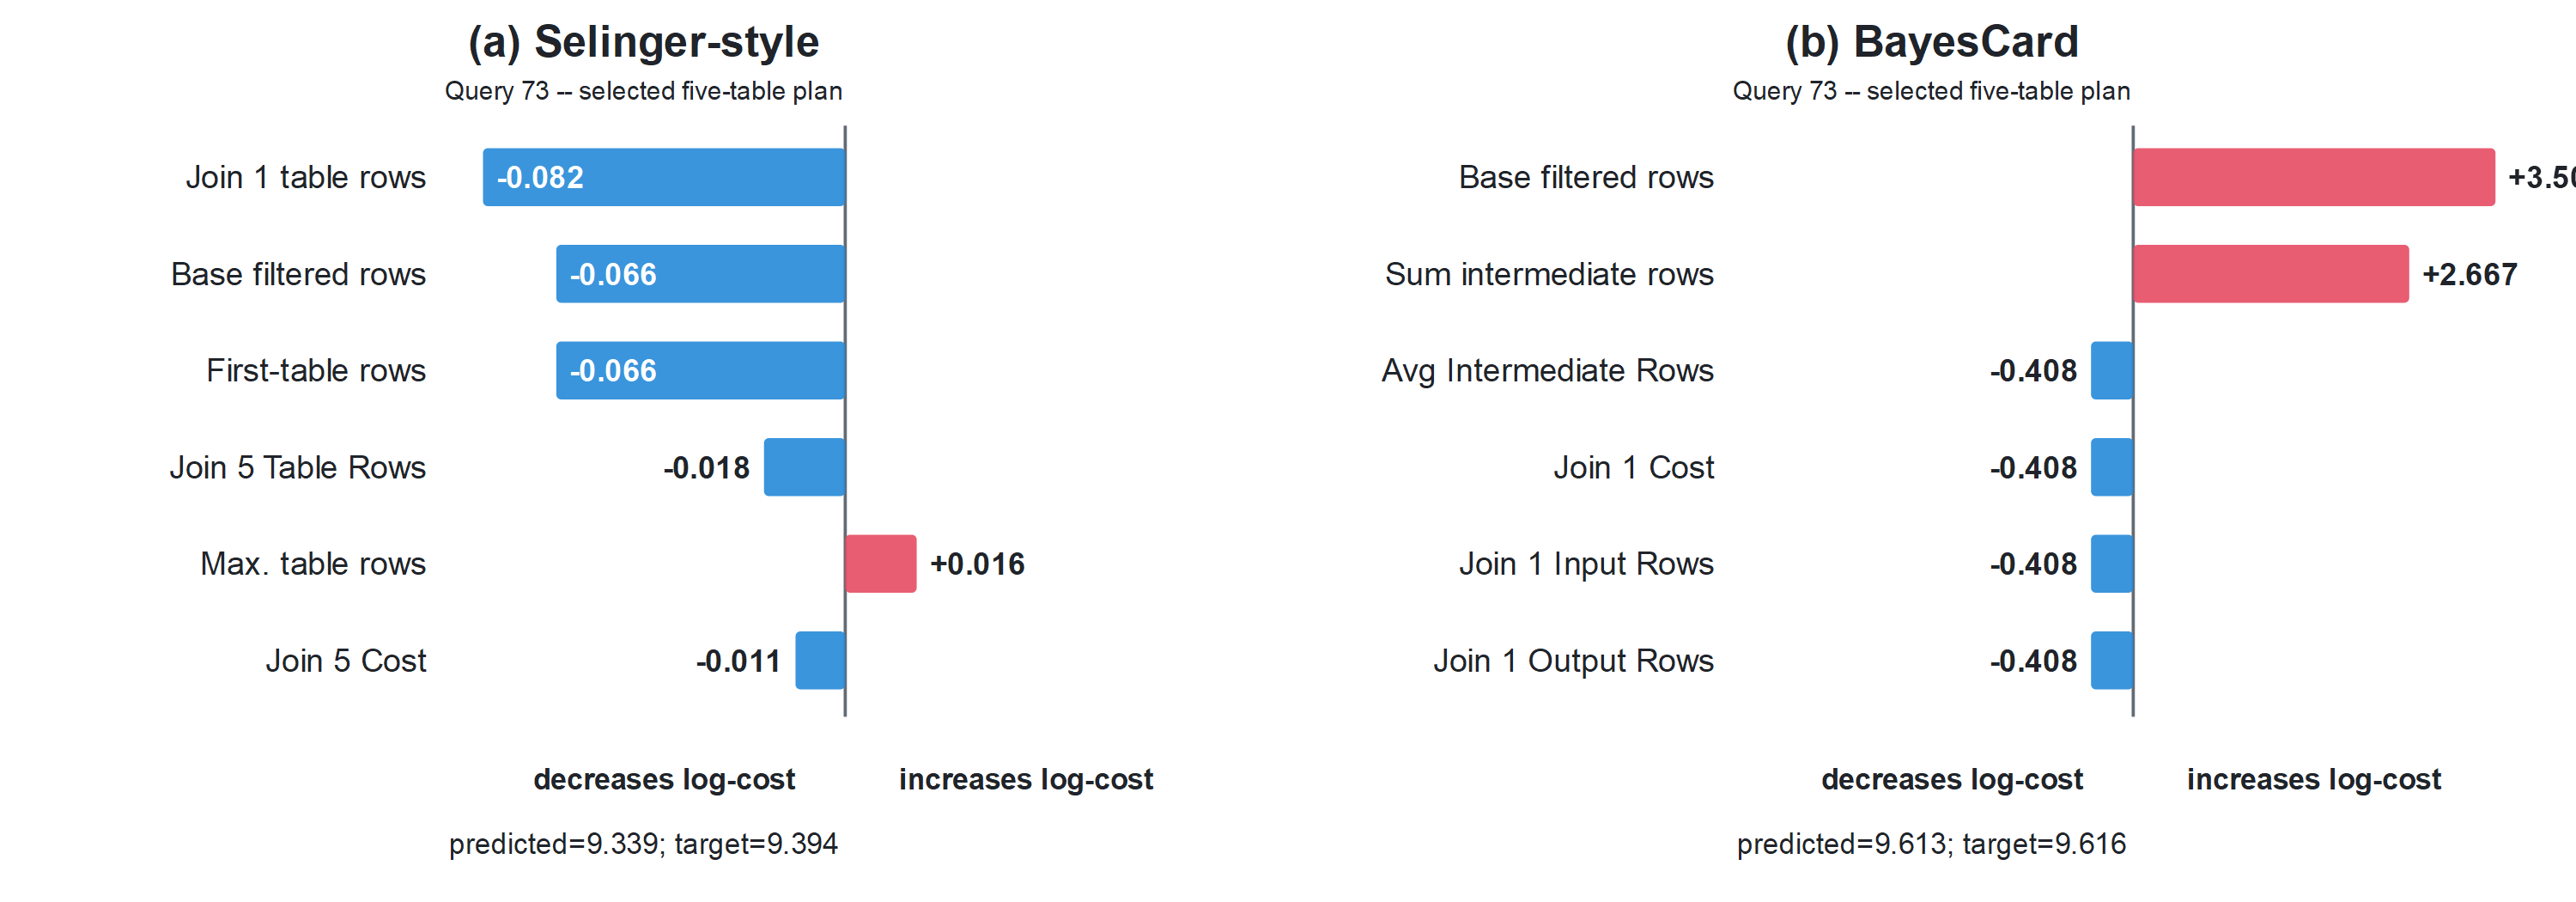
\includegraphics[width=0.90\textwidth]{fig3_local_shap.png}
  \caption{Local SHAP contributions for selected plans of the same five-table query, in surrogate log-cost space. Red increases and blue decreases predicted optimizer cost.}
  \label{fig:local_shap}
\end{figure*}

The 112 templates, 45 configurations, and two optimizers produced 10,080 query-configuration observations. Five-table queries yielded 48 Selinger and 24 BayesCard plans, while both reached the 50-plan cap at six tables (Table~\ref{tab:workload}), substantially enlarging the original plan sets.

\subsection{Ridge Surrogate Fidelity}

The out-of-query evaluation shows that Ridge closely approximates both cost models. Across size-distribution conditions, Selinger obtained mean $R^2$ of 0.9929--0.9932 and log-MAE of 0.0212--0.0228; BayesCard obtained 0.9962--0.9998 and 0.0150--0.0555, respectively (Table~\ref{tab:fidelity}).

Selinger's Kendall $\tau$ was 0.9009--0.9053 and top-1 agreement 0.6250--0.6375. BayesCard rank metrics are N/A because nearly all candidate target costs were tied; assigning zero would misrepresent an undefined ordering as failure.

\begin{table}[htbp]
\caption{Out-of-query Ridge surrogate fidelity}
\label{tab:fidelity}
\centering
\scriptsize
\resizebox{\columnwidth}{!}{%
\begin{tabular}{lcccc}
\toprule
\textbf{Optimizer} & \textbf{$R^2$} & \textbf{Log-MAE} & \textbf{Kendall $\tau$} & \textbf{Top-1} \\
\midrule
Selinger & 0.9929--0.9932 & 0.0212--0.0228 & 0.9009--0.9053 & 0.6250--0.6375 \\
BayesCard & 0.9962--0.9998 & 0.0150--0.0555 & N/A & N/A \\
\bottomrule
\end{tabular}%
}
\end{table}

Condition-level means and 95\% intervals are retained in the experiment outputs.

\subsection{Global Feature Attribution and Stability}

Fig.~\ref{fig:shap_stability} shows that the optimizers retain the distinct profiles observed in the original study. Selinger produces a distributed importance profile, consistent with its broader search space and sensitivity to multiple structural features. Its leading features were \texttt{max\_table\_rows} (8.64\%), \texttt{join\_1\_table\_rows} (7.98\%), \texttt{base\_filtered\_rows} (6.60\%), and \texttt{first\_table\_rows} (6.60\%). In contrast, BayesCard concentrates importance on \texttt{base\_filtered\_rows} (33.89\%) and \texttt{sum\_intermediate\_rows} (27.88\%), consistent with the constraint that fixes its initial table.

Stability was evaluated per query over the five seeds, sizes, and distributions. Fig.~\ref{fig:shap_stability} reports mean normalized importance with bootstrap 95\% confidence intervals; the complete outputs additionally retain standard deviation, mean rank, and top-5 frequency.

\subsection{Local and Comparative Explanations}

To understand individual decisions, the framework generates local SHAP waterfall explanations for the selected plans (Fig.~\ref{fig:local_shap}). Each plot decomposes the optimizer's cost estimate from the expected base cost; red contributions push estimated cost higher and blue contributions push it lower. The contrastive view compares the selected plan with its closest alternative, clarifying why one sequence of intermediate joins was preferred over another.

For human-readable inspection, a Large Language Model receives the structured SHAP explanation and produces an executive summary of the main positive and negative cost drivers together with a comparison against the runner-up plan. The LLM is invoked only after the quantitative explanation has been computed and cannot affect plan enumeration, cost estimation, Ridge fitting, or feature attribution.

Combining SHAP visualizations with natural-language summaries provides quantitative and human-readable views of optimizer decisions. Their practical usefulness for DBAs is a potential application, not a result established here; it requires a controlled study with real users.


\subsection{Estimated vs. Runtime Validation}

Runtime tracing revealed that the estimated intermediate cardinalities driving optimizer decisions did not always match observed execution. Nevertheless, their relative magnitudes often remained informative. SHAP explains why the optimizer assigned a cost, whereas q-error exposes discrepancies between the estimates and physical execution; a large q-error can therefore identify a weakness in cardinality estimation without implying a failure of the Ridge proxy.


\subsection{Proof-of-Concept Scalability}

XAI preparation was measured per query as an initial proof-of-concept scalability check. For six-table queries, BayesCard required 102.93 ms on average and Selinger 477.23 ms; their p95 peak memory was 444.33 and 455.77 KiB, respectively. These prototype measurements use a 50-plan cap and do not demonstrate production scalability. Evaluating time and memory on larger workloads remains future work.


\subsection{Threats to Validity}

The synthetic six-table star schema was designed to isolate optimizer behavior and may not generalize to production workloads. The engine and optimizers are research prototypes, and the 50-plan cap truncates the six-table search spaces. Some Selinger results were identical across seeds and distributions because its evaluated cost features were insensitive to those changes; zero-width intervals are therefore implementation-specific, not evidence of universal stability. The study includes neither a DBA user evaluation nor learned, adaptive, or production optimizers.


\FloatBarrier
\section{Conclusions}

This work presented an exploratory framework for improving the transparency of cost-based SQL query optimization through XAI techniques. By vectorizing execution plans into interpretable numerical features and applying SHAP through a local Ridge proxy, the approach quantifies how plan characteristics contribute to the optimizer's estimated cost and produces both global and local explanations.

The expanded experiment preserves the original qualitative distinction between the optimizers: Selinger distributes cost sensitivity across several structural features, whereas BayesCard concentrates it on base filtering and intermediate rows. The auxiliary fidelity evaluation shows that Ridge closely approximates the prototype cost models, and the repeated experiment quantifies SHAP variability across seeds, sizes, and distributions with 95\% confidence intervals. Runtime q-error remains a complementary diagnostic of discrepancies between estimated and observed quantities.

These results are proof-of-concept evidence from a controlled synthetic environment, not a demonstration of production scalability or improved DBA decisions. Future work should evaluate JOB or TPC-H, larger plan spaces, modern learned or adaptive optimizers, additional XAI techniques such as LIME, and the usefulness of visual and natural-language explanations through controlled studies with database professionals.


\begin{thebibliography}{00}

\bibitem{b1} P. G. Selinger, M. M. Astrahan, D. D. Chamberlin, R. A. Lorie, and T. G. Price, ``Access path selection in a relational database management system,'' in \textit{Proc. ACM SIGMOD}, 1979, pp. 23--34.

\bibitem{b2} G. Graefe, ``Query evaluation techniques for large databases,'' \textit{ACM Comput. Surv.}, vol. 25, no. 2, pp. 73--169, 1993.

\bibitem{b3} H. Lan, Z. Bao, and Y. Peng, ``A survey on advancing the DBMS query optimizer: Cardinality estimation, cost model, and plan enumeration,'' \textit{Data Sci. Eng.}, vol. 6, no. 1, pp. 86--101, 2021.

\bibitem{b4} V. Leis, A. Gubichev, A. Kemper, and T. Neumann, ``How good are query optimizers, really?'' \textit{Proc. VLDB Endow.}, vol. 9, no. 3, pp. 204--215, 2015.

\bibitem{b5} G. Moerkotte, T. Neumann, and G. Steidl, ``Preventing bad plans by bounding the impact of cardinality estimation errors,'' \textit{Proc. VLDB Endow.}, vol. 2, no. 1, pp. 982--993, 2009.

\bibitem{b6} L. Getoor, B. Taskar, and D. Koller, ``Selectivity estimation using probabilistic models,'' in \textit{Proc. ACM SIGMOD}, 2001.

\bibitem{b7} A. Kipf, T. Kipf, B. Radke, V. Leis, P. Boncz, and A. Kemper, ``Learned cardinalities: Estimating correlated joins with deep learning,'' in \textit{Proc. CIDR}, 2019.

\bibitem{b8} R. Marcus et al., ``Neo: A learned query optimizer,'' \textit{Proc. VLDB Endow.}, vol. 12, no. 11, pp. 1705--1718, 2019.

\bibitem{b9} Y. Han, Z. Wu, Z. Yang, R. Zhu, and J. Zhou, ``Are we ready for learned cardinality estimation?'' \textit{Proc. VLDB Endow.}, vol. 15, no. 9, pp. 1640--1654, 2022.

\bibitem{b10} Z. Wu, A. Shaikhha, R. Zhu, K. Zeng, Y. Han, and J. Zhou, ``BayesCard: Revitalizing Bayesian frameworks for cardinality estimation,'' arXiv:2012.14743, 2020.

\bibitem{b11} R. Guidotti, A. Monreale, S. Ruggieri, F. Turini, F. Giannotti, and D. Pedreschi, ``A survey of methods for explaining black box models,'' \textit{ACM Comput. Surv.}, vol. 51, no. 5, pp. 1--42, 2018.

\bibitem{b12} M. T. Ribeiro, S. Singh, and C. Guestrin, ``Why should I trust you?: Explaining the predictions of any classifier,'' in \textit{Proc. ACM SIGKDD}, 2016.

\bibitem{b13} S. M. Lundberg and S.-I. Lee, ``A unified approach to interpreting model predictions,'' in \textit{Adv. Neural Inf. Process. Syst.}, vol. 30, 2017.

\bibitem{b14} R. Marcus and O. Papaemmanouil, ``Deep reinforcement learning for join order optimization,'' in \textit{Proc. Workshop Data Management for End-to-End Machine Learning}, 2018, pp. 1--4.

\end{thebibliography}

\end{document}
